% this TeX file provides an awesome example of how TeX will make super 
% awesome tables, at the cost of your of what happens when you try to make a
% table that is very complicated.
% Originally turned in for Dr. Nico's Security Class
\documentclass[11pt]{article}
\usepackage[a4,margin=1in]{geometry}


\usepackage[utf8]{inputenc}
\usepackage{graphicx}
\usepackage{tikz}
\def\checkmark{\tikz\fill[scale=0.4](0,.35) -- (.25,0) -- (1,.7) -- (.25,.15) -- cycle;} 

% multirow allows you to combine rows in columns
%\usepackage{multirow}
% tabularx allows manual tweaking of column width
\usepackage{tabularx}
% longtable does better format for tables that span pages
\usepackage{longtable}

\begin{document}
\setlength{\parindent}{0pt}
% this is an alternate method of creating a title
%\hfill\vbox{\hbox{Gius, Mark}
%       \hbox{Cpe 456, Section 01}  
%       \hbox{Lab 1}    
%       \hbox{\today}}\par
%
%\bigskip
%\centerline{\Large\bf Lab 1: Security Audit}\par
%\bigskip
\author{Grégoire Hirt\\ Marc Bickel\\ Raphaël Barman}
\title{\vspace{-2.0cm}Report: Part 3}
\maketitle
\vspace{-1cm}
\section{State of the project}
Let's begin with a screenshot:
\begin{center}
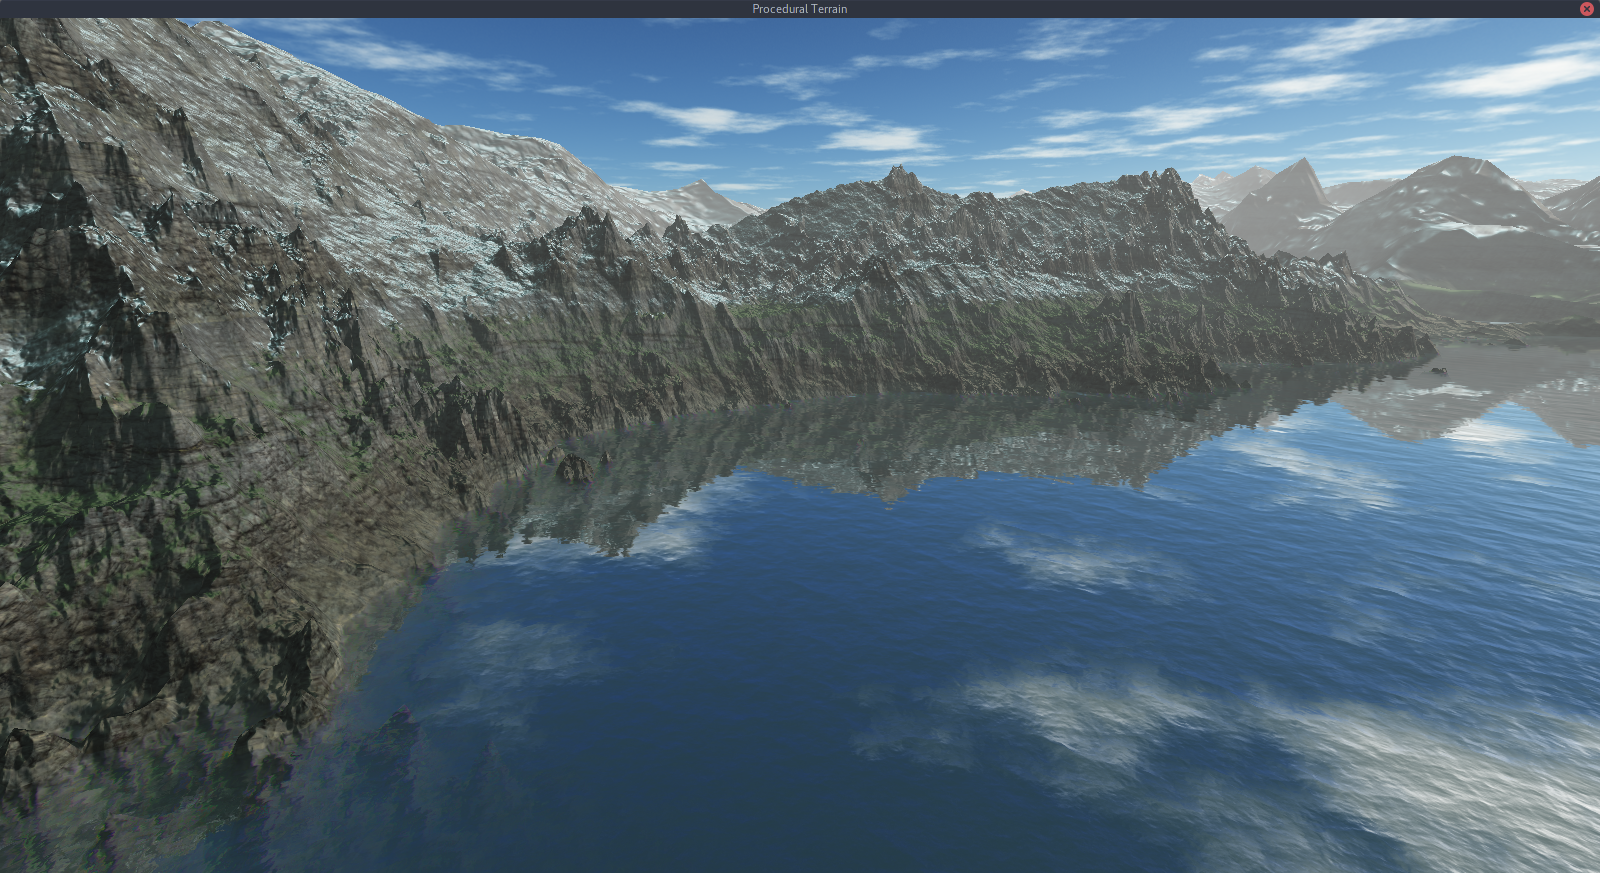
\includegraphics[width=\textwidth]{screen04}
\caption{Current state of the project}
\end{center} \\

What we implemented during this third part was:
\begin{itemize}
\end{itemize}

\begin{center}
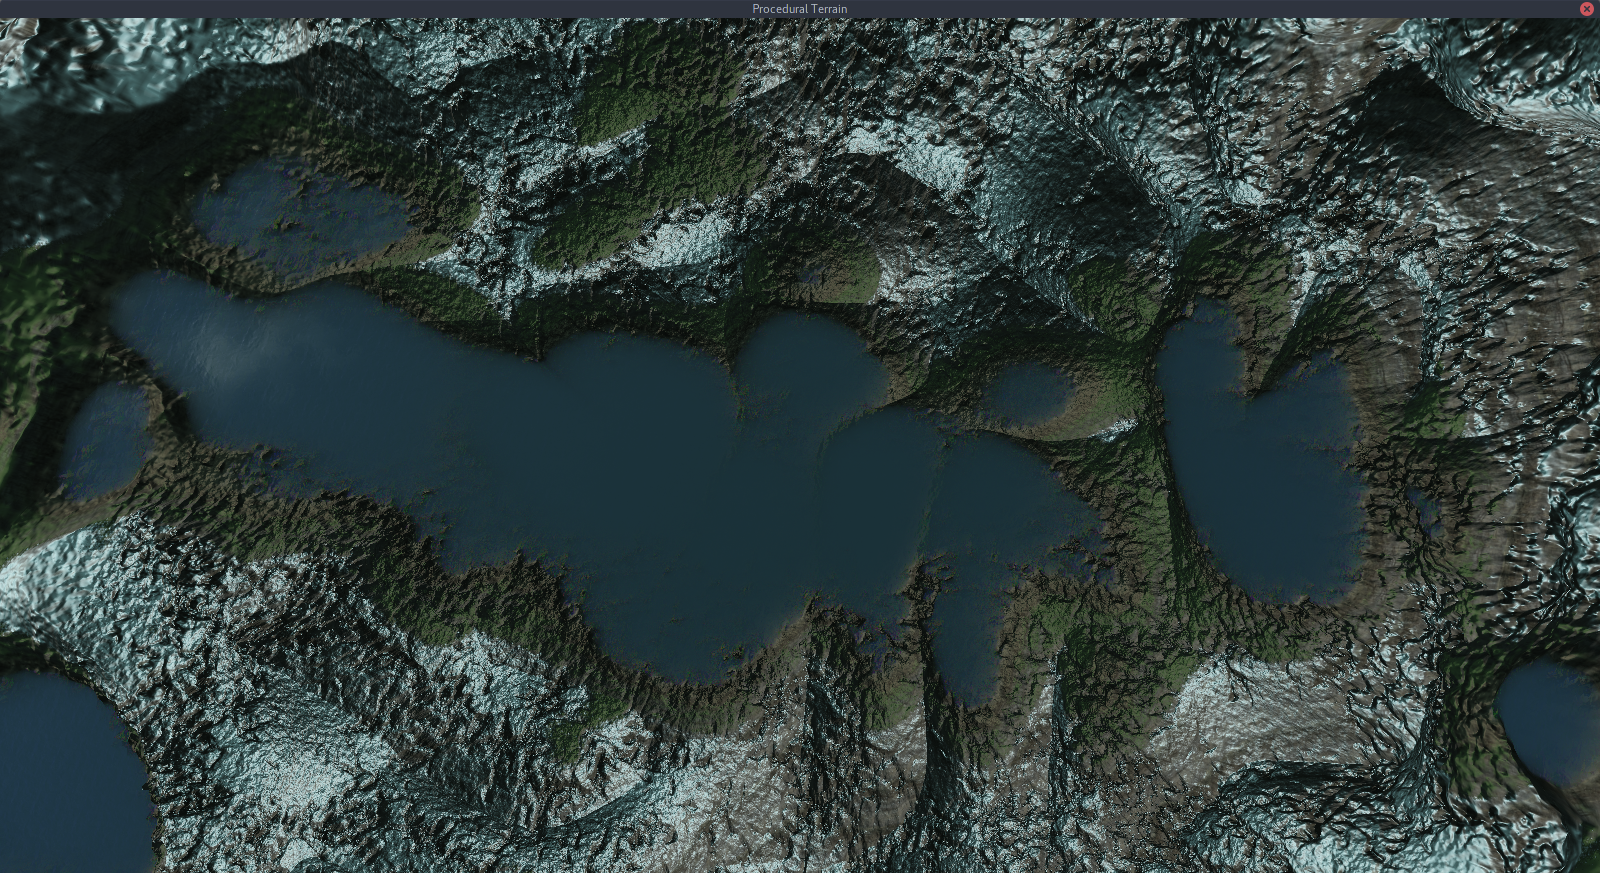
\includegraphics[width=\textwidth]{screen05}
\caption{Top view}
\end{center} 

We will now explain in details the implementation of the previously mentioned
parts. 

\subsection{Triplanar texturing}

We updated the terrain fragment shaders to feature a decent Phong lighting and
triplanar texturing. This also include fragment-wise evaluation of the heightmap
to add bump-mapping to the terrain. This allow to achieve fairly detailed
landscape without pushing the vertex count to high. We then use a power of the
dot product between the up-vector and the terrain normal in model space to
compute the 'slope' of the ground. Based on this slope we then map either the
flat surface texture or the sloppy surface texture (top or rock). The top
texture also change depending on the altitude this is done by re-using the 1D
texture with the colors at different height from the previous part and them
mapping colors to the amount of each texture.

\subsection{Water rendering}

\subsubsection{Reflective water}

To achieve reflexion, we used the same technique as in one of the assignments,
rendering the seen flipped upside-down by multiplying view matrix by a mirror
matrix. We then use the resulting texture as a color for the water surface. The
problem with this approach is that underwater terrain also gets rendered and
seems to hover over water. To address this, we added a clip plane at the surface
of the water to avoid underwater terrain to render in the mirror. 

\subsubsection{Full fresnel model water}

The water was great this way but we wanted to have some more details. So we now
render the terrain in a dedicated framebuffer instead of the window directly.
This allow to use this back texture as a color for adding refractions to  the
water. The water color is then blended between reflection and refractions using
an approximated fresnel model based on the normal of the water surface and the
view angle. Another thing that we added is a water fog. Meaning that when we see
the water from above, the luminosity of the refractions are decreasing with
depth, and underwater becomes almost black from a certain threshold. Of course,
deformation of the reflexion and refraction images are approximations since we
have planar texture and not environment maps that would be less efficient. So
we use the difference between flat reflected vector and distorted reflected
vector as an offset in the texture lookup. Same goes for the refraction.

A small bonus feature is the chromatic aberration based on the water depth.
Meaning red green and blue components don't get distorted exactly the same way
and give this impression of colored blur.

Of course the water surface is given some specular factor to add some shine over
the waves.

\subsection{Skybox}

The skybox was implemented in a quite canonical way. By loading 6 faces of a cube
map in a CubeMap Texture and then using the normalized vertex coordinates in a
zero centered cube to lookup the texture. We also disable depth writing to
prevent the skybox, which is drawn first, to occlude the terrain. To keep the
skybox centered on the camera we simply zero-out the last column of the view
matrix when drawing the skybox. This cancels only translation and thus preserve
rotation and scale (scale not needed but since we don't scale the view it does
not matter).

\subsection{Multithreaded noise generation}

Since noise generation became a big part of the project, noise sampling was
taking down the framerate when we were switching back and forth. At first,
we implemented a job queue to process each chunk update on a different frame.
This way the payload was distributed across many frames and we saw fps
improvement, but this was not enough. So we decided to take the noise generation
to a shared Opengl context that's running in another thread. This way we can
generate textures without disturbing terrain rendering. The chunks then simply
wait for future textures to be ready and cross-fade them with the previous one
(that could be higher or lower resolution depending on the way we are moving the
camera). This system gave some trouble to tune, because we didn't want to have
the worker thread to busy-wait on an empty job queue, so we had to find the best
heuristics to make the thread sleep.

\begin{center}
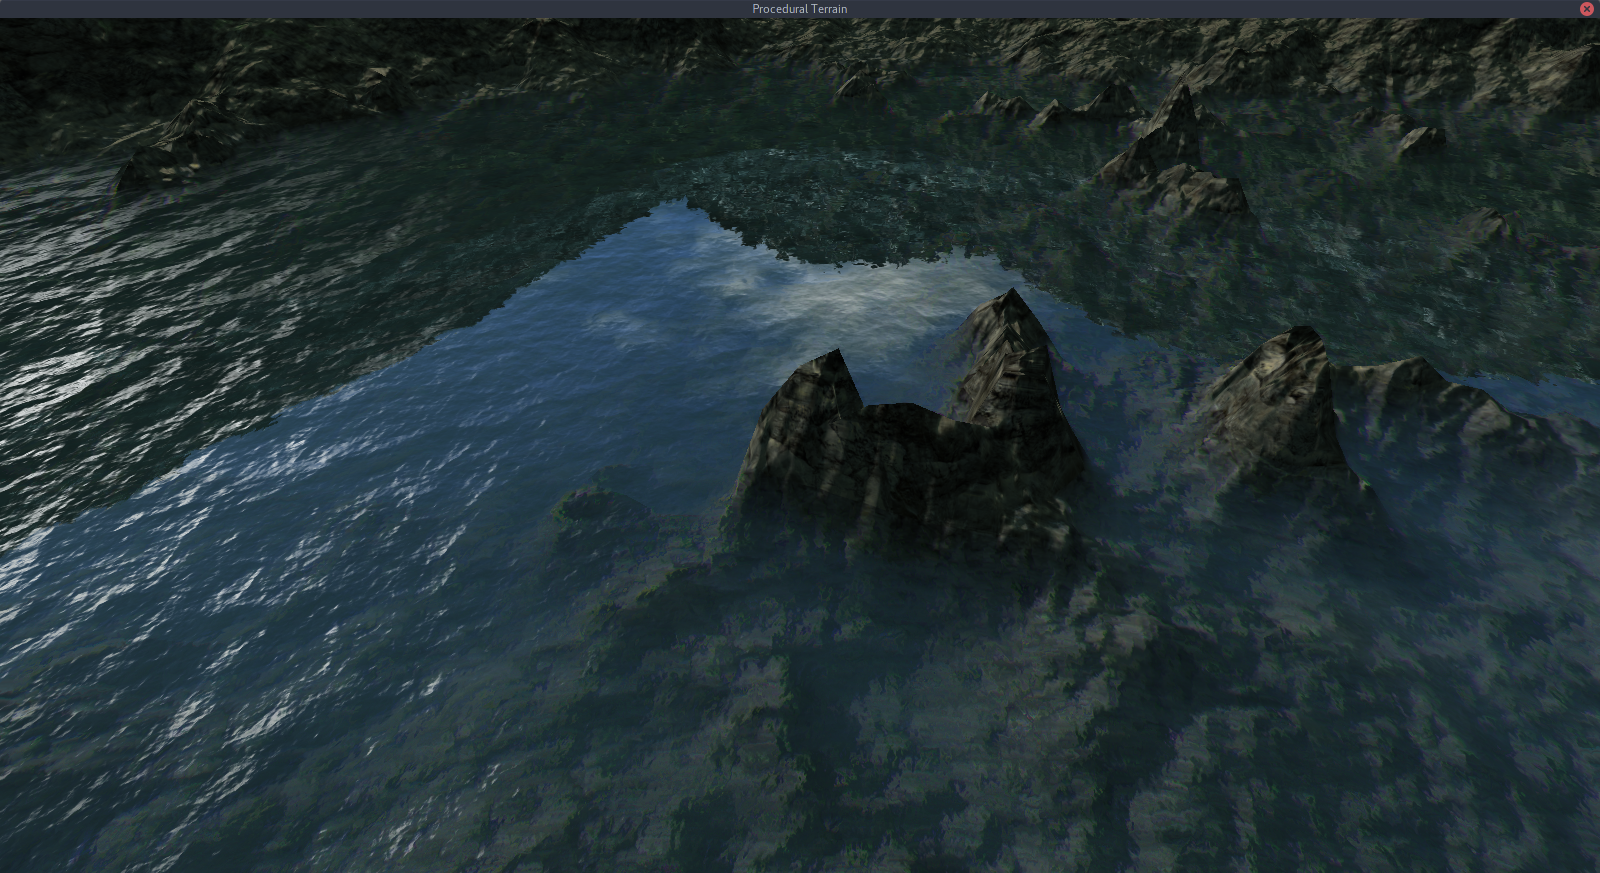
\includegraphics[width=\textwidth]{screen06}
\caption{Advanced water}
\end{center} \\

\section{Work distribution}
\subsection{Mandatory part}

\begin{tabular}{l|ccc}
 & Marc & Grégoire & Raphaël \\ \hline
Texturing & \checkmark  & \checkmark & \checkmark \\
Basic water &\checkmark  &  & \checkmark \\
Skybox & \checkmark  &  & \checkmark  \\
\end{tabular}

\subsection{Extra part}

\begin{tabular}{l|ccc}
 & Marc & Grégoire & Raphaël \\ \hline
Triplanar texturing & \checkmark & \checkmark & & \\
Multithreaded noise generation & &  \checkmark & &  \\
Advanced water & &\checkmark  & \checkmark & \\
\end{tabular}

\end{document}
